% $Id: preview.tex,v 1.19 1998/06/22 08:07:00 ohl Exp $
%%%%%%%%%%%%%%%%%%%%%%%%%%%%%%%%%%%%%%%%%%%%%%%%%%%%%%%%%%%%%%%%%%%%%%%%


\NeedsTeXFormat{LaTeX2e}
\documentclass[11pt]{article}
\usepackage{amsmath,amssymb,amsthm}
\usepackage[margin=1.0in]{geometry}
\usepackage{amscd}
\usepackage{amsthm}
\usepackage{epsfig}
\allowdisplaybreaks
\setlength{\unitlength}{1mm}
%%%%%%%%%%%%%%%%%%%%%%%%%%%%%%%%%%%%%%%%%%%%%%%%%%%%%%%%%%%%%%%%%%%%%%%%
\makeindex
\begin{document}
\title{\bf {PURE DATA SPACES....DRAFT...DRAFT...DRAFT}}
\author{%
  SAUL YOUSSEF%
  \hfil \\
  Department of Physics \\
  Boston University \\
}
\maketitle
\begin{abstract}
All about spaces.
\end{abstract}
%%%%%%%%%%%%%%%%%%%%%%%%%%%%%%%%%%%%%%%%%%%%%%%%%%%%%%%%%%%%%%%%%%%%%%%%

%%%%%%%%%%%%%%%%%%%%%%%%%%%%%%%%%%%%%%%%%%%%%%%%%%%%%%%%%%%%%%%%%%%%%%%%
\theoremstyle{definition}
\newtheorem{axiom}{Axiom}
\newtheorem*{axiom*}{Axiom}
\newtheorem*{fact}{Fact}

\newtheorem{definition}{Definition}

\newtheorem*{remark}{}

\section{Overview}

In Reference 1, we introduced an axiomatic framework, based on the finite sequence as the foundational concept.  
With finite sequences assumed, we had 
\begin{itemize}
\item[1 ]{\it ``Data" is a finite sequence of ``codas,'' where each coda is a pair of data.}
\end{itemize}
\noindent This kind of data, such as (:)\ (:(:))\ ((:):(:)\ (:)), is ``pure data'' in the sense that it is ''made of nothing.'' Such data has two natural operations: 
{\it concatenation} of data A with data B, written (A\ B), and {\it pairing} data A and data B as a {\it coda}, written (A:B).  
\begin{itemize}
\item[2 ]{\it Definitions are embodied by a chosen partial function $\delta$ from codas to data called a context.}
\end{itemize}
As modest as it is, 1 and 2 appear to be able to capture Mathematics in general.  Consequences include:   
\begin{itemize}
\item[-]{Fixed points of $\delta$ ({\it atoms}), represent fixed data such as bits, bytes and text;}
\item[-]{Data outside the domain of $\delta$ are {\it variables}, which might become defined over time as {\it definitions} are added to $\delta$;} 
\item[-]{$\delta$ contains it's own {\it language}, allowing user specification of data and adding definitions to $\delta$;} 
\item[-]{Equality of data A=B is determined by $c\sim\delta(c)$ and by compatibility with finite sequences. Proof and computation are then defined by the equality.  A sequence $A_1=A_2=\dots=A_n$ is both a proof of $A_n$ given $A_1$ and a computation $A_1\mapsto A_n$.  Proof and computation are essentially the same thing;}
\item[-]{Data is {\it true} if it is empty, {\it false} if it is atomic, and {\it undecided} otherwise.  Undecided data may also be {\it undecidable}, as in the Godel phenomena or other seeming paradoxes.  Data which is {\it never false} as definitions are added is a {\it theorem}.}
\end{itemize}

In this work, we investigate the concept of a {\it space}, introduced in Reference 1.  


...SEARCHING....ORGANICS....

\section{Foundation}  

In \cite{PDF}, we argue that Mathematics and Computing as a whole can be captured within a small axiomatic framework, 
based on {\bf finite sequence} as the foundational concept.  Assuming that finite sequences are understood, {\it data} and {\it coda} are defined by 

\begin{definition} {{\bf Data} is a finite sequence of {\bf codas}, where each {\bf coda} is a pair of {\bf data}.}
\end{definition}

\noindent The two foundational operations defined on data are 1) concatenation of data $A$ and data $B$, written `$A\ B$', and 2) pairing of data $A$ and data $B$ as a coda, written with a colon `$A:B$'.   
By Definition 1, the empty sequence, written `()', qualifies as data and, therefore, () paired with itself is a coda, written `(():())' or `(:)'.  
Any finite sequence of codas is data, so, for example, (:)\ (:(:))\ ((:):(:(:))) is  
data consisting of a sequence of three codas.  We can think of this as {\it pure data} since it is ``data made of nothing.''  
By convention, the colon binds from the right first and binds less strongly than concatenation, so that $A:B:C$ is defined to be $(A:(B:C))$ and $A:B\ C$ is defined to be $(A:(B\ C))$.  
Data is typically written with upper case, and codas are typically written in lower case.  
To indicate the left and right data of a coda, we sometimes use L/R superscripts so, for any coda $c$, $c=(c^L:c^R)$. 

     All meaning within the system is determined by a chosen partial function from coda to data called a {\it context}. 
Contexts are partially ordered by inclusion, so if $\delta$ and $\delta'$ are contexts, $\delta\le\delta'$ if $\delta$ and $\delta'$ are equal on the domain of $\delta$.  
Given a context $\delta$, equality of data is the equivalence generated by $c\sim \delta(c)$ for any coda $c$, and by compatibility with concatenation and colon in the sense that 
if $A\sim B$, then $(A\ X)\sim (B\ X)$, $(X\ A)\sim (X\ B)$, $(A:X)\sim (B:X)$ and $(X:A)\sim(X:B)$ for any data $X$.  This relation $A\sim B$ is denoted $A{\overset\delta =}B$, 
or simply $A=B$ when the context is unambiguous.   
It follows that if $\delta\leq\delta'$, then $A{\overset\delta =}B$ implies $A{\overset{\delta'} =}B$.  We say that if $A$ and $B$ are equal then they are ``always equal,'' thinking 
of moving from $\delta$ to $\delta'$ as the passage of ``time."  The fixed points of a context $\delta$ are {\it atoms}.  Note that if $c$ is an atom in context $\delta$, 
and if $\delta\leq\delta'$, then $c$ is still an atom a context in $\delta'$.  Thus, atoms are ``permanent" and if $c$ is an atom, $c$ is ``always" an atom.  

\begin{definition}
{Within a given context $\delta$, coda $c$ is an {\bf atom} if $\delta:c\mapsto c$.  If data $A$ contains an atom in its sequence, $A$ is {\bf atomic} data. 
Data $A$ is {\bf invariant} if every coda $a$ in the sequence of $A$ is an atom and if $a^L$ and $a^R$ are both {\bf invariant}. }
\end{definition}
\noindent It follows from the definition that empty data is invariant and atoms $a$ and $b$ are equal if and only if $a^L=b^L$ and $a^R=b^R$.  If $a$ and $b$ are atoms, 
$A$ and $B$ are data, then $(a\ A)=(b\ B)$ and $(A\ a)=(B\ b)$, if and only if $a=b$ and $A=B$.  If $A=B$ and $A$ and $B$ are invariant, then $A$ and 
$B$ are identical as pure data [proof].

\section{Genesis}

    In the proposed framework, all mathematical objects are pure data and all meaning is defined by a chosen context $\delta$ and its corresponding equivalence.  
A {\bf proof} in $\delta$, for example, is just a sequence $A_1{\overset \delta =}$ $A_2 {\overset \delta =} \dots {\overset \delta =}$$A_n$ which can be viewed either as proving $A_n$ 
given $A_1$ or as a computation $A_1\mapsto A_n$. 
The immediate issue is how to choose $\delta$.  
    
     In the beginning, there are no definitions, and the corresponding context is the empty partial function $\delta_0$.  
Since the domain of $\delta_0$ is empty, it has no fixed points and, therefore no atoms.  Thus, the empty sequence is the only invariant, 
$X{\overset \delta =}X$ is the only valid proof, and the only valid 
 computations do nothing $X\mapsto X$ for any data $X$.
To define a non-empty context $\delta_0\le\delta$, we need, at least, an invariant specification of the domain of $\delta$ as a partial function.    
Since the empty sequence is the only invariant, the only way to specify if a coda (A:B) is to be in the domain of $\delta$ is 
to require either A or B or both to be the empty sequence. In each of these cases, the coda (:) is within the domain of $\delta$, and so we must, in any case, 
decide on what (:) maps to.  There are three possibilities; 
\begin{itemize}
\item[] choice 1: {$\delta: (:) \mapsto ()$},
\item[] choice 2: {$\delta: (:) \mapsto (:)$}, or 
\item[] choice 3: {$\delta: (:) \mapsto \ anything\ other\ than\ ()\ or\ (:)$}. 
\end{itemize}
Since pure data is ``made of (:)'', choice 1 trivially causes all data to be equal to the empty sequence. 
On the other hand, choice 3 would mean that for any non-empty data $A$, the number of (:) atoms in $A$ grows without limit.  This would mean, for instance, 
that nocomputation could produce a final result.  Thus, we are constrained to choice 2, where (:) is an invariant atom in $\delta$, and, therefore an atom in 
any context $\delta\leq\delta'$ as well.  It is convenient to generalize choice 2 and to let $\delta$:(:$X$)$\mapsto$ (:$X$) for all data $X$, since this provides a 
supply of invariant atoms (:), (:(:)), (:(:) (:)),$\dots$ which can be used to expand the domain of $\delta$.  

We adopt a convention for expanding the domain of $\delta$ while preserving context partial ordering. 
A context of the form 
\begin{equation}
	\delta_a: (a\ A:B) \mapsto \delta_a(A,B)
\end{equation}
for some invariant atom $a$ is called a {\bf definition}.  We conventionally restrict ourselves to 
contexts $\delta\cup\delta_a\cup\delta_b\cup\dots$ where $a$ is an invariant atom in $\delta$, $b$ is an invariant atom in $\delta\cup\delta_a$, $c$ is an invariant atom in $\delta\cup\delta_a\cup\delta_b$ and so forth.  By requiring $a$, $b$,\dots to be disjoint, we maintain the context partial ordering.  

\section{Definitions}

     Before proceeding to mathematical exploration, we need to add enough expressive power to the original context $\delta$.  To do this, 
we introduce minimal definitions using the mechanism explained in the previous section.  

\begin{enumerate}
\item {Define ``bits'', ``bytes'' and ``byte sequences'' so that words are single atoms, so that $a$ can be a word in future definitions $\delta_a$.}
\item {Define all of the naturally occurring combinatoric operations given two finite sequences $A$ and $B$.  For example $\delta_{\rm ap}$
maps (ap $A$ : b$_1$\ b$_2$ $\dots$ b$_n$) to ($A$:b$_1$)\ ($A$:b$_2$)$\dots$ ($A$:b$_n$), so that ap ``applies $A$ to each atom of input.'' }
\item {Define a minimal internal language $\delta_{\{\}}$ so that a coda $(\{\texttt{language expression}\}\ A : B)$ is mapped to data as described by 
the expression and possibly using data $A$ and data $B$.}
\item {Include definitions giving direct access to context-level values.  This include a Boolean definition $\delta_{\rm bool}$ to determine if data is empty, 
$\delta_{=}$ to test if two data are equal in $\delta$, and $\delta_{\rm def}$ to add definitions via Equation 1.} 
\end{enumerate}
There are approximately fifty definitions needed to cover basic system function and combinatorics, making a minimal convenient context for mathematics.  
We will list a few of these here.  A complete list can be found 
in the Glossary.  

\subsection{Bits, Bytes and Byte sequences}

For convenience, we first define atomic {\it bits}, {\it bytes}, and {\it byte sequences}, so that we can make 
more readable definitions.  Define 
\begin{itemize}
\item{$\delta_{(:)}$ : single bit atoms, so that ((:):), ((:):(:)) are the zero bit and the one bit respectively.}
\item{$\delta_{((:):)}$ : atoms containing eight bits.}
\item{$\delta_{((:):(:))}$ : atoms containing arbitrary length byte sequences.}
\end{itemize}
so, for instance, text strings are atomic data within $\delta\cup\delta_{(:)}\cup\delta_{((:):)}\cup\delta_{((:):(:))}$.  

\subsection{Combinatorics} 

Given that text strings are now invariant atoms, we can add definitions with readable names.  Define the identity `pass' so that (${\rm pass}:X$=$X$) for all data $X$.  
\begin{itemize}
\item{$\delta_{\rm pass}$ : ({\rm pass} A:B) $\mapsto$ B}
\end{itemize}
and define `null' so that (${\rm null}:X$=$()$) for all $X$.
\begin{itemize}
\item{$\delta_{\rm null}$ : ({\rm null} A:B) $\mapsto$ ()}
\end{itemize}
It is convenient to define ``getting the A and B components of a coda'' like so
\begin{itemize}
\item{$\delta_{\rm left}$ : ({\rm left} A:B) $\mapsto$ A} 
\item{$\delta_{\rm right}$ : ({\rm right} A:B) $\mapsto$ B} 
\item{$\delta_{\rm put}$ : ({\rm put} A:B) $\mapsto$ (A:B)}
\item{$\delta_{\rm get}$ : ({\rm get} : (:B)) $\mapsto$ B} FIX ME
\end{itemize}
We proceed to define the minimal combinatorics involving of A and B as finite sequences.  These don't have 
commonly understood names, so we are forced to invent new names.  For example the name `ap' is meant to suggest the 
concept ``apply A to each atom of B" is expressed by the definition.  
\begin{itemize}
\item{$\delta_{\rm ap}$ : ({\rm ap} A : b B) $\mapsto$ (A:b) ({\rm ap} A : B)}
\item{$\delta_{\rm ap}$ : ({\rm ap} A : ()) $\mapsto$ ()} 
\end{itemize} 
The domain of $\delta_{\rm ap}$ is defined with the assumption that $b$ is an atom, so the domain of the first branch of $\delta_{\rm ap}$ is exactly 
codas $({\rm ap}\ A,B)$ where $B$ starts with an atom.  By definition, if we list multiple ``branches'' as in this case, the first branch in the domain applies.  

\subsection{Language} 

Axiomatic systems like ZFC[ref] or dependent type theories[ref] are formal languages.  There is an alphabet, special symbols, and syntax rules 
for defining valid expressions.  Our approach avoids this by defining a language as just one more definition like any other.  The basic idea is to 
define minimalist language, mainly giving access to the two basic operations via text blank space and text colon.  So, the basic idea is 
\begin{itemize}
\item {$\delta_{\{\}}$ : (\{x\ y\} A : B) $\mapsto$ (\{x\} A:B) (\{y\} A:B)}
\item {$\delta_{\{\}}$ : (\{x:y\} A : B) $\mapsto$ (\{x\} A:B) : (\{y\} A:B)}
\end{itemize}
where x and y are byte sequences as defined above.  As written, this is ambiguous since $x$ and $y$ may contain space and colon characters, but 
these ambiguities can easily be resolved by choosing and order in the text string and by ordering the above, thus forcing the language into one definition 
$\delta_{\{\}}$.  This definition includes 
\begin{itemize}
\item {$\delta_{\{\}}$ : (\{A\} A : B) $\mapsto$ A}
\item {$\delta_{\{\}}$ : (\{B\} A : B) $\mapsto$ B}
\end{itemize}
so that A and B have special meaning in the language.  As a result, for example, (\{B\}:1 2 3)=1 2 3, (\{B B\}:1 2 3)=1 2 3 1 2 3, and (\{A B\} a b : 1 2)=a b 1 2.  

     Given a language expression in the form of byte sequence data $L$, the corresponding data is, simply, ($L$:).  Every sequence of bytes is a valid language 
expression, so there is actually no need to define or check for syntax errors.  Similarly, an {\it evaluation} of ($L$:) is merely some sequence 
($L$:)=$D_1$=$D_2$=$\dots$=$D_n$ producing an ``answer'' $D_n$.  Typically, this is done with a simple strategy based on applying $\delta$ whenever 
possible or up to time or space limits.  This also means that there is also no such thing as a ``run time error.''    

\subsection{System} 

    The most basic question to ask about data is whether it is empty or not.  This is captured by the definition $\delta_{\rm bool}$, defined 
so that (bool:B) is () if B is empty (``true'') and (bool:B)=(:) if B is atomic (``false'').
\begin{itemize}
\item {$\delta_{\rm bool}$ : ({\rm bool} A : B) $\mapsto$ () if $B$ is empty, (:) if $B$ is atomic.}
\item {$\delta_{\rm not}$ : ({\rm not} A : B) $\mapsto$ (:) if $B$ is empty, () if $B$ is atomic.} 
\end{itemize} 
The equality defined by the context $\delta$ is available within $\delta$ via the following definition:
\begin{itemize}
\item {$\delta_{=}$ : (= A : ()) $\mapsto$ A}
\item {$\delta_{=}$ : (= (): A) $\mapsto$ A}
\end{itemize}
and if a and b are atoms, 
\begin{itemize}
\item {$\delta_{=}$ : (= a A : b B) $\mapsto$ (= a:b) (=A:B)}
\item {$\delta_{=}$ : (= A a : B b) $\mapsto$ (=A:B) (= a:b)}
\end{itemize}
so, if $(A:B)$ is empty, $A$ and $B$ are ``always'' equal and if $(A:B)$ is atomic, $A$ and $B$ are ``never'' equal.  The full language has a little bit 
of syntactic sugar, so one can write (A=B) instead of (= A:B) [ref]. 

New definitions can also be added to context via  
\begin{itemize}
\item {$\delta_{def}$ : ({\rm def} \texttt{name} A : B} $\mapsto$ ())
\end{itemize}
which is defined to be in domain as a partial function if \texttt{name} is not already in the current context, and, in that case, it adds the following definition
to context.
\begin{itemize}
\item {$\delta_{\texttt{name}}$:(\texttt{name}\ $A'$:$B'$) $\mapsto$ ($B\ A'$:$B'$)}
\end{itemize}
so, for instance (def first2 : {first 2 : B}), means that (first2 : a b c d) is interpreted as (\{first 2:B\} : a b c d) which is equal to the data (a b).   

We take this as the ``organic'' base of naturally occurring 
definitions plus the language will be a starting point in searching for the ``spaces'' defined in section 5.  Further definitions used in the text can be found in 
the Glossary.  Examples, tutorials, a complete definition of the language, and software can be 
found in reference [x]. 

\section{Global Structure} 

    Pure data has a global structure in the sense that the foundational operations $(A\ B)$ and $(A:B)$ are defined for any data $A$, $B$.  
This suggests defining a corresponding associative product $(A\cdot B)$ and associative sum $(A+B)$ by    
\begin{equation}
(A \cdot B):X = A:B:X 
\end{equation}
\begin{equation}
(A+B):X = (A:X)\ (B:X) 
\end{equation}
for all data $X$.  Since $({\rm pass}\cdot A)$=$(A\cdot {\rm pass})$=$A$ and $(A+{\rm null})$=$({\rm null}+A)$=$A$ for any $A$, pure data is a {\it semiring} with units pass and null.  
Following standard terminology, we say that $A$ is {\it idempotent} if $A\cdot A$=$A$, is an {\it involution} if $A\cdot A$=$1$, and $A$ has an {\it inverse} if $A\cdot A'$=$A'\cdot A$=$1$ for some data $A'$.   
In the case of a {\it product}  A=$A_n\cdot\dots\cdot A_1$, we say that A {\it starts with} $A_1$ and {\it ends with} $A_n$.   

Data $A$ is {\it commutative} if $A:X\ Y$=$A:Y\ X$ for all $X$, $Y$, and is {\it distributive} if $A:X\ Y$=$(A:X)\ (A:Y)$ for all $X$ and for all $Y$.  
The concepts of commutative and distributive data are complementary in a sense that foreshadows later sections where we investigate `spaces.'  
Commutative data can be expected to be ``mathematical'' because such data has, in a sense, transcended the finite sequence concept and might be 
expected to have a Platonic meaning beyond this particular system.  We shall see multiple examples.  Distributive data, on the other hand, is strongly 
sequence dependent, but is also interesting mathematically because it such data is, in a sense a ``morphism of finite sequences."  To emphasize this theme, we will sometimes refer 
to commutative data as {\it algebraic} data and will sometimes refer to distributive data as a {\it homomorphism}. 

Any data $A$ can be viewed as defining a binary operation on data defined by ($X{\overset A\ast}Y)=(A:X\ Y)$.  Since ${\overset A\ast}$ is associative if and only if 
 (A:X\ Y)=(A:(A:X)\ Y)=(A:X (A:Y)) for all X,Y we say that data $A$ is {\it associative} if it has this property.  

     If we say that data $A\leq B$ if $A\cdot B=A$, this defines a global preorder structure on data where 
$\leq$ is transitive in general and reflexive on idempotents.  For example, null$\leq X\leq$pass for any data $X$.  
The equivalence $A\leq B$ and $B\leq A$ is indicated by saying that $A$ and $B$ are {\it compatible} data.
 
\section{Spaces}

      A very basic requirement for useful mathematics is to have a way to define and refer to collections.  In classical mathematics, this 
need is met by the concept of a Set.  In the framework of pure data, every mathematical object must be identified with some data, and this must include any sort of collection of mathematical objects.  
Thus, we are lead to ask, given some data $S$, how could $S$ represent a collection of other data?  
There are a couple of plausible ways to do this.  
\begin{enumerate} 
\item The collection corresponding to $S$ would be the data ($S$:$X$) for any data $X$.
\item The collection corresponding to $S$ would be all of the fixed points of $S$.  
\end{enumerate}
These two ideas coincide if we require $S$ to be idempotent, so that ($S:X$) is always a fixed point.  It is natural to also expect compatibility with 
sequences in the sense that if ($S:X$) is in the collection and ($S:Y$) is in the collection, then ($S:X$) ($S:Y$) is also in the collection.  
This is guaranteed if we require 
\begin{equation}
(S : X\ Y) = S : (S:X)\ (S:Y)
\end{equation}
for all data $X$, $Y$.  
These requirements are neatly satisfied if $S$ is associative, since associative data is idempotent and also always satisfies 
Equation 4.  Thus, we are lead to a simple definition.  
\begin{definition} Data $S$ is a {\bf space} if $S$ is associative.
\end{definition}
\noindent If $S$ is a space, we say that any data ($S$:$X$) is {\it in} $S$.  
The data ($S$:) is called the {\it neutral data} of $S$ and a space where ($S$:)=() is called a {\it neutral} space.  
It is easy to verify that if spaces $S$ and $T$ commute, then $S\cdot T$ is 
also a space and from the preorder perspective of Section 5, any data compatible with a space is itself a space. 

Many of the basic definitions are spaces, including `pass', `null', `bool' from section 4 and others, as shown in figure X.  
More examples come from noting that any data which is both idempotent and distributive is also a space.  Thus if $J$ is idempotent data, then 
(ap\ $J$) is idempotent and distributive, and is, therefore, a space.    

\subsection{Morphisms} 

A product $F$ that starts with space $S$ and ends with space $T$ is a {\it morphism} from $S$ to $T$ and can be written $S{\overset F\longrightarrow}T$.
A morphism $F$ always defines a function mapping ($S:X$) in $S$ to ($T:F:X$) in $T$.  Since spaces are idempotent, $F\cdot S$=$T\cdot F$=$F$.  Since the product of data is 
associative, morphisms can be composed as usual, so that if $S{\overset F\longrightarrow}T$ and 
$T{\overset G\longrightarrow}U$, then $S{\overset {G\cdot F}\longrightarrow}U$.  

     It is helpful to think of morphisms from $S$ to $S$ as belonging to $S$, and so we will refer to a morphism $S{\overset f\longrightarrow}S$ as a morphism ``of $S$'' and we may indicate this as $f\in S$.
Morphisms of a space $S$ have a semiring structure which is a slight generalization of the global semiring from Section 5.  Given morphisms $f, g\in S$, we have a semiring with 
product $f\cdot g$, and with associative sum $f\oplus g$, defined to be $S\cdot (f+g) \cdot S$.  
Distribution from the right follows as before, so $(f\oplus g)\cdot h = (f\cdot h)\oplus (g\cdot h)$ for all $f,g,h\in$S.  
Multiplicative and additive units are inherited via $1$=$S\cdot${\rm pass}$\cdot S$=$S$ and $0$=$S\cdot${\rm null}$\cdot S$, so that 
$1\cdot f$=$f\cdot 1$=$f$ and $0\oplus f$=$f\oplus 0$=$f$ for all $f\in$S.  For any morphism $f\in S$, $0\cdot f=0$.  
Since every space $S$ is also a product of spaces starting at $S$ and ending at $S$, every space $S$ also qualifies as a morphism from $S$ to itself ($S{\overset S\rightarrow}S$).

Given a space $S$, we can identify a number of distinguished classes of morphisms within the semiring of $S$. 
\begin{itemize}

\item{{\bf Subspaces.} If a morphism $f\in S$ happens to also be a space, we say that $f$ is a {\it subspace} of $S$.  The name ``subspace'' is justified because every data contained in $f$ is also contained in S, and every morphism $f\cdot$X$\cdot f$ of $f$ is also a morphism of $S$.  Algebraically, subspaces partially distribute from the left as 
in $f\cdot(g\oplus h)=f\cdot((f\cdot g)\oplus(f\cdot h))$.  Every space has subspaces $1$ (the whole space), $0$ (just the neutral data of the space) and every data ($S$:$X$) in $S$ has a corresponding 
constant subspace morphism.} 

\item{{\bf Homomorphisms.} If a morphism $f$ is distributive, we say that $f$ is a {\it homomorphism} of S.  
Homomorphisms distribute both from the left as well as the right, so that $f\cdot(g\oplus h)=(f\cdot g)\oplus(f\cdot h)$ if $f$ is a homomorphism.  If $f$ and $g$ are 
homomorphisms, so is $f\cdot g$.}

\item {{\bf The Group of units}. The collection of morphisms $g\in$S with multiplicative inverses ($g\cdot g'=g'\cdot g=1$) is called {\it the group of units} of the space $S$.  
The group of units may including {\it involutions} where $g\cdot g=1$.  As usual, involutions $g$ and $h$ commute if and only if $g\cdot h$ is also an involution.  Data in $S$ which is invariant under the group of units is 
called {\it central} data.  Morphisms which commute with the group of units are called {\it central} morphisms.}

\item {{\bf Algebraic Morphisms.} The morphisms of an algebraic space are automatically algebraic as well.  In general, if $f,g\in$S and $f$ is algebraic, then $g\cdot f$ is algebraic.  If both 
$f$ and $g$ are algebraic, $f\oplus g$ is algebraic.}

\item{{\bf Neutrality} A morphism $f\in S$ {\it preserves neutrality} if ($f$:$S$:)=($S$:) and {\it reflects neutrality} if ($f$:$S$:$X$)=($S$:) implies ($S$:$X$)=($S$:). 
The morphisms which preserve neutrality are exactly the morphisms which satisfy $f\cdot 0$=$f$ in addition to satisfying $0\cdot f=0$.  Since 0 and 1 preserve neutrality, 
and since ($f\cdot g$) and ($f\oplus g$) preserve neutrality if $f$ and $g$ do, neutrality preserving morphisms are a subsemiring of $S$.  If $f\in S$ and $g\in S$ reflect neutrality, 
then so does $f\cdot g$.  A morphism $f\in S$ is a {\it positive morphism} if ($f$:$X$) is never equal to the neutral data of $S$.  If $f$ and $g$ are positive in $S$, then so is $f\cdot g$ and, 
if $S$ itself is neutral, $f\oplus g$ is also a positive morphism.}  
\end{itemize} 
Since the morphisms of $S$ always include a constant subspace for each data $S:X$ in $S$, the collection of morphisms of $S$ is strictly richer 
than the data contents of $S$.  We shall see that it is fruitful to think of a space $S$ as its collection of endomorphisms. 

\subsection{Subspaces are substructures} 

Suppose that space $S$ has subspace $s$ and space $T$ has subspace $t$, and suppose that $F$=$t\cdot X\cdot s$ is a morphism from $s$ to $t$.   
Since ($t\cdot X\cdot s$) = ($T\cdot t \cdot X\cdot s\cdot S$), 
$F$ is also a morphism from $S$ to $T$, with the extra property that $F$ respects the structure of $s$ and $t$ in the sense that $t\cdot F=F\cdot s$ (figure X).
\begin{figure}[h]
\centering
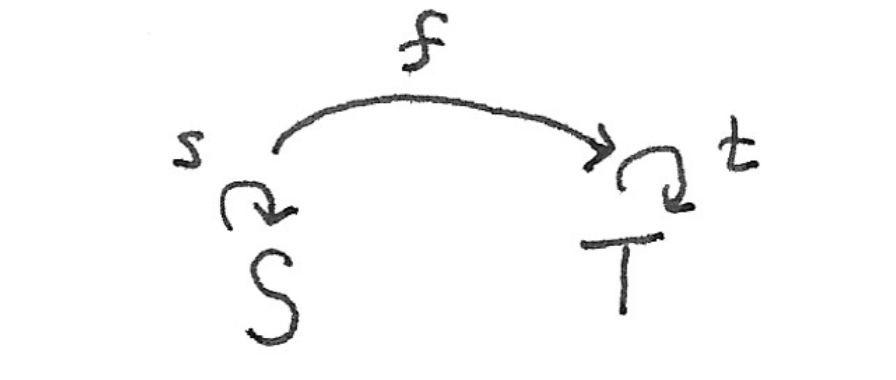
\includegraphics[width=0.3\textwidth]{subspace.png}
\caption{{\it Subspaces are substructures.  If s is a subspace of S and t is a subspace of T, then a morphism from s to t is
a morphism from S to T which preserves the corresponding structure.}}
\end{figure}
Since the morphisms of $S$ automatically includes a constant subspace for each data $(S:X)$ in $S$, the morphisms of $S$ are strictly richer than the contents of $S$.  

\subsection{Isomorphisms} 

Borrowing a definition from category theory, spaces $S$ and $T$ are {\it isomorphic} if the diagram in Figure X commutes for 
some morphisms $\alpha$ and $\alpha'$, where $S$ and $T$ serve as their own ``identity morphisms.''  It easily follows that 
the semirings of S and T are isomorphic as monoids, and thus, have the same idempotents, involutions, group of units and identity.  
If $\alpha$ and $\alpha'$ are homomorphisms, we say that $S$ and $T$ are {\it homeomorphic}.  In this case, 
the semirings of $S$ and $T$ are isomorphic as semirings. 
\begin{figure}[h]
\centering
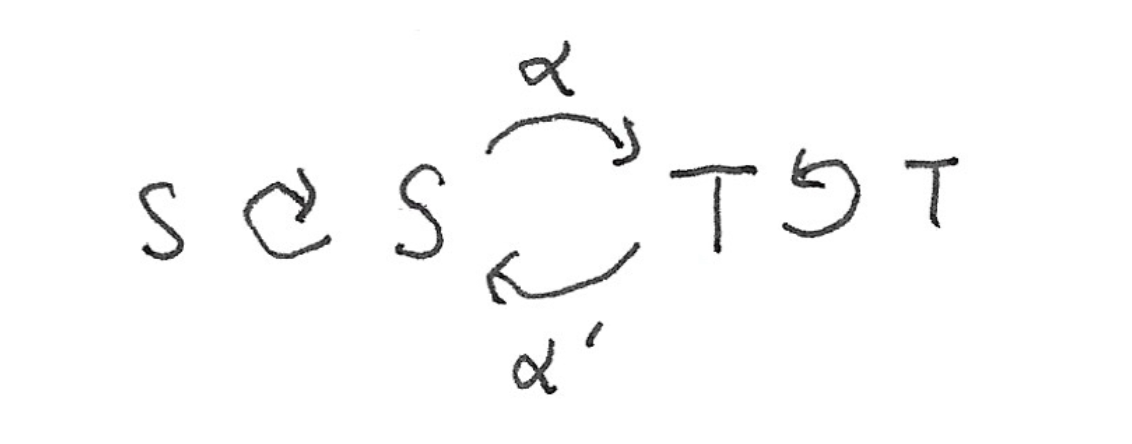
\includegraphics[width=0.4\textwidth]{isomorphism.png}
\caption{{\it In a definition adopted from Category Theory, spaces S and T are isomorphic if the diagram commutes, using S and T themselves instead of identity morphisms.}}
\end{figure}

The basic theory of spaces and morphisms gives us enough of a framework to investigate spaces.  Our strategy is first look at the spaces which emerge most 
simply, ``organically'' and naturally from the space of all pure data.

\subsection{Organic Spaces}

   Since the general concept of a collection leads directly to Definition 3, it is clear that spaces must play a fundamental role 
in the mathematics of pure data, perhaps in a way analogous to the role that Sets or Categories play in classical mathematics. However, it is also 
clear that spaces are quite different from either Sets or Categories.  Most basically, a set is defined by its contents and a space is not.  For example,
the space (ap \{a\}) contains the same data as (is a), but these spaces are not equal.  
Since a space always contains its neutral data ($S$:), unlike a set, a space can never be empty.  An implicit operation mapping 
($S$:$X$) and ($S$:$Y$) to ($S$:$X$\ $Y$), means that spaces come with a richer internal structure than Sets.  
Although spaces have morphisms and associative composition, the theory of spaces must also be quite different than Category Theory because, for example, morphisms exist 
between any two spaces.  
These considerations suggests that pure data spaces may provide a different, and possibly interesting perspective on known mathematics.  
This possibility informs the strategy of the rest of this paper.  We 
search for the simplest, most natural, most ``organic'' spaces, understand them in the context of the structures above, and compare with known mathematics.  

    The pure data framework gives us some advantages in searching for the ``simplest'' spaces, since we could search all pure data and find all spaces 
up to a specified maximum data width and depth.  This direct approach is computationally difficult, but we can proceed in this spirit, by starting with 
the basic definitions which also happen to be spaces, some of which are shown in figure X.   We can take the point of view that we let 
spaces ``grow organically'' from the space of all pure data and examine the simplest results first.  
\begin{figure}[h]
\centering
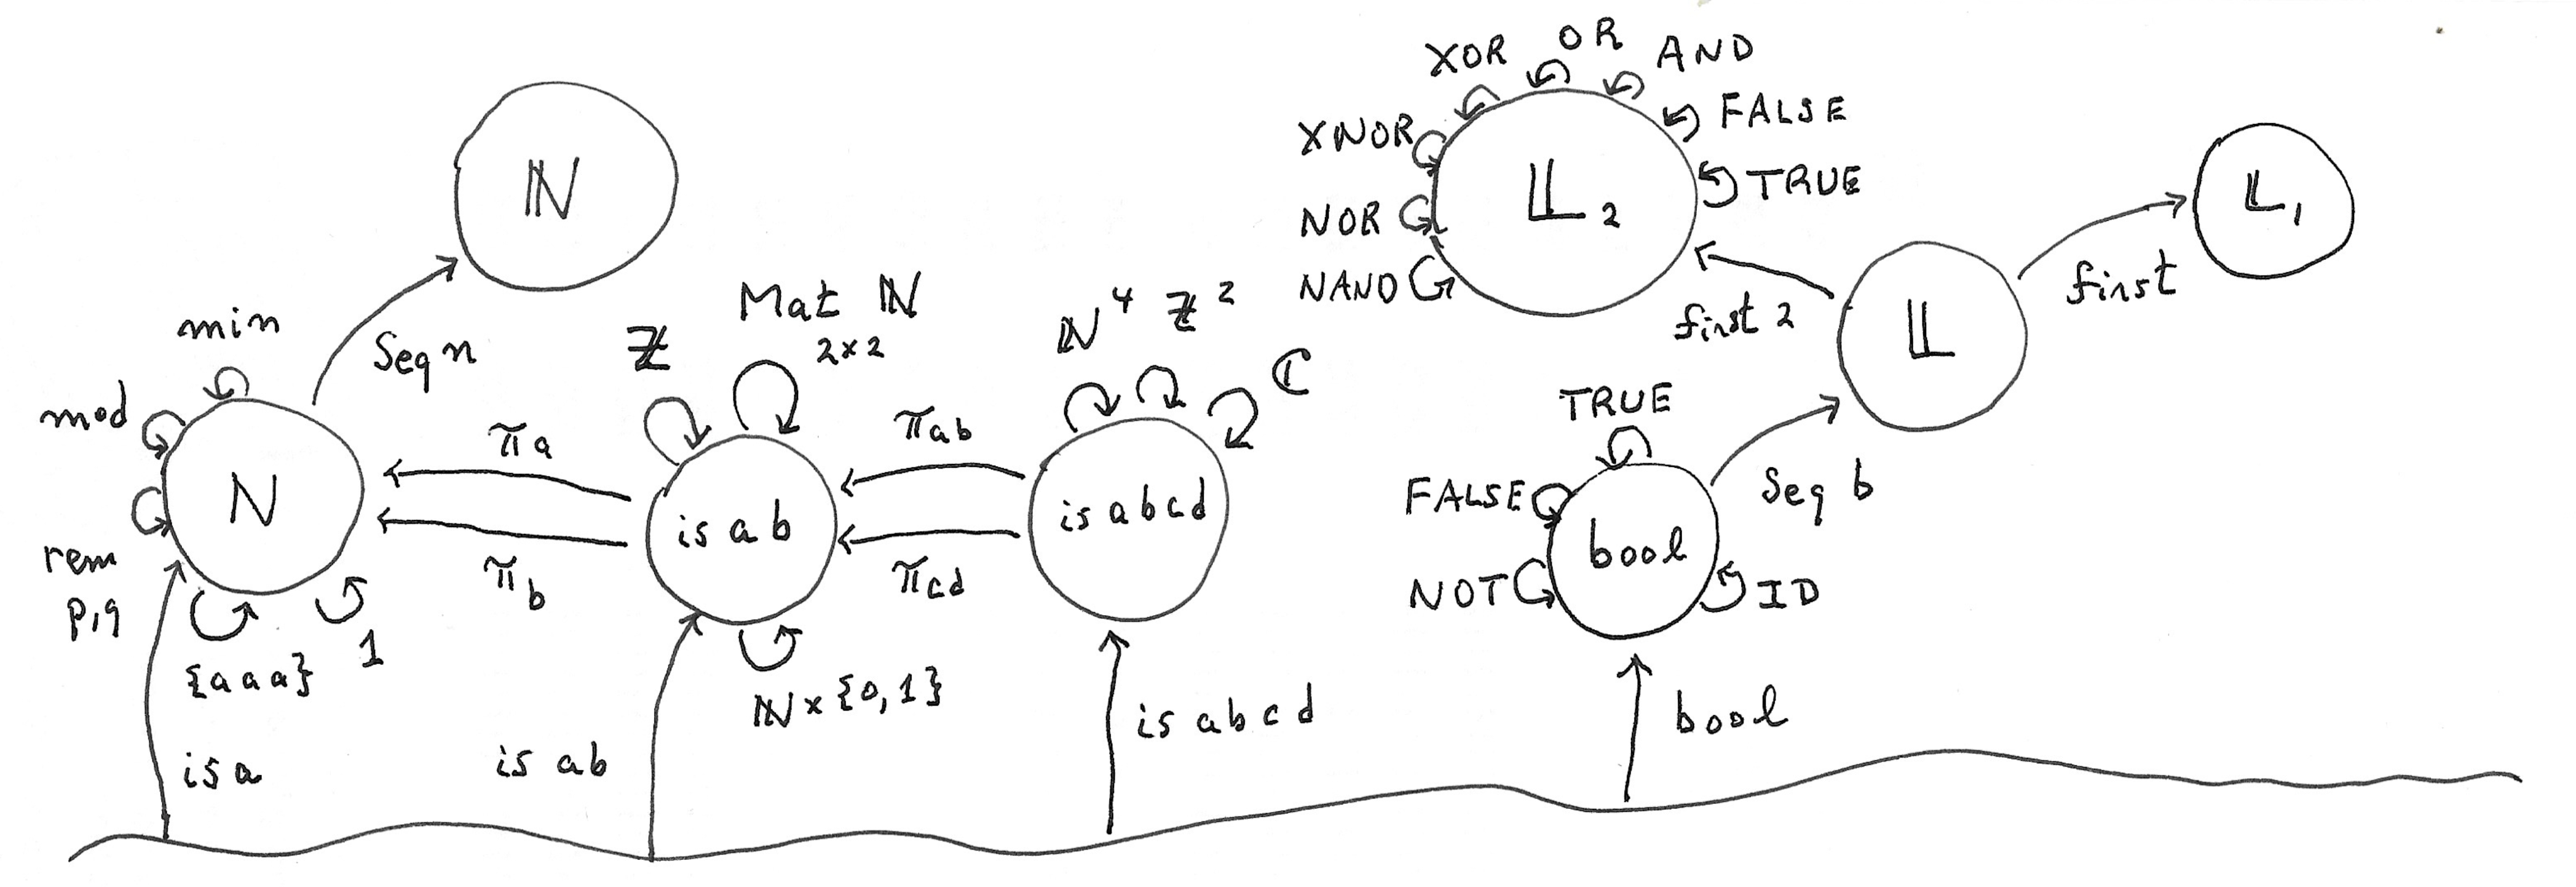
\includegraphics[width=0.6\textwidth]{garden.png}
\caption{{\it The space of all pure data contains all mathematical objects.  Our strategy for exploring this space is to first introduce 
the minimal combinatorics implicit from the foundational finite sequence concept, and then examine the simplest spaces first as they 
appear ``organically.''  Since algebraic spaces are commutative, they, in a sense, transcend the foundational sequence concept and are more ``Platonic.''}}
\end{figure}
Aside from the ``organic'' theme, a second theme is to take special notice of `algebraic' data to see how this matches with the intuition that 
algebraic spaces and morphisms will be the most mathematically significant, worthy of special naming, and the most Platonic in the sense
of being independent of this particular system.  

\section{The Space of all data} 

     Since spaces are fixed points on their contents, any space that contains all data, must be a fixed point on all data, and so the distributive space `pass` is 
the unique space containing all pure data.  We shall think of spaces as ``growing from the garden'' of pure data, in other words, from the 
contents of pass. 

Before growing the simplest spaces, it helps to orient ourselves by examining the semiring structure of `pass' itself.  The multiplicative and 
additive identities of pass are $1$=pass$\cdot$pass$\cdot$pass=pass, and $0$=pass$\cdot$null$\cdot$pass=null respectively.  Note that every data 
$X$ is actually a morphism of pass, since $X$=pass$\cdot X\cdot$pass.  Consider the classes of morphism defined in Section 6. 
\begin{itemize}
\item{{\bf Subspaces.}  Since every data is a morphism of pass, every space is a subspace of pass.}
\item{{\bf Homomorphisms.} By definition, the homomorphisms of pass are the distributive data $D$ with the property $D$:$X$\ $Y$=($D$:$X$)\ ($D$:$Y$).}
\item{{\bf The Group of Units.} The units of pass are the permutations such as (swap 1 2) and (rev).  Central data are data consisting of a sequence of 
identical atoms, such as (:) (:) (:), or (a a a), which can be interpreted as the ``organic number three."}
\item{{\bf Algebraic Morphisms.} Since algebraic morphisms commute with permutations, all algebraic morphisms are central in pass. 
Morphisms like (ap const (:)) or (is a) are algebraic homomorphisms of pass and are, thus, distinguished as ``Platonic'' spaces with
mathematical significance.  In this case, they each represent the natural numbers.}
\item{{\bf Neutrality.} A morphism D$\in$pass is neutral preserving if ($D$:)=(), is neutral reflecting if ($D$:$X$=()) implies $X=()$ 
and is positive if ($D$:$X$) is never empty.  For example,
\begin{itemize}
\item[-] pass, rev, first, \{B B\}, (is a) are neutral preserving.
\item[-] pass, rev, first, are neutral reflecting.
\item[-] const 1 2 3, \{\#\}, \{B 1 2 3\} are positive. 
\end{itemize}
}
\end{itemize}

As an example of an isomorphism, consider the isomorphism pass$\cong$has illustrated in Figure X.  This isomorphism $X\leftrightarrow(:X)$ embodies 
``storing and retrieving data $X$''.  A similar isomorphism $X\leftrightarrow(a:X)$ exists for every atom $a$.   

\begin{figure}[h]
\centering
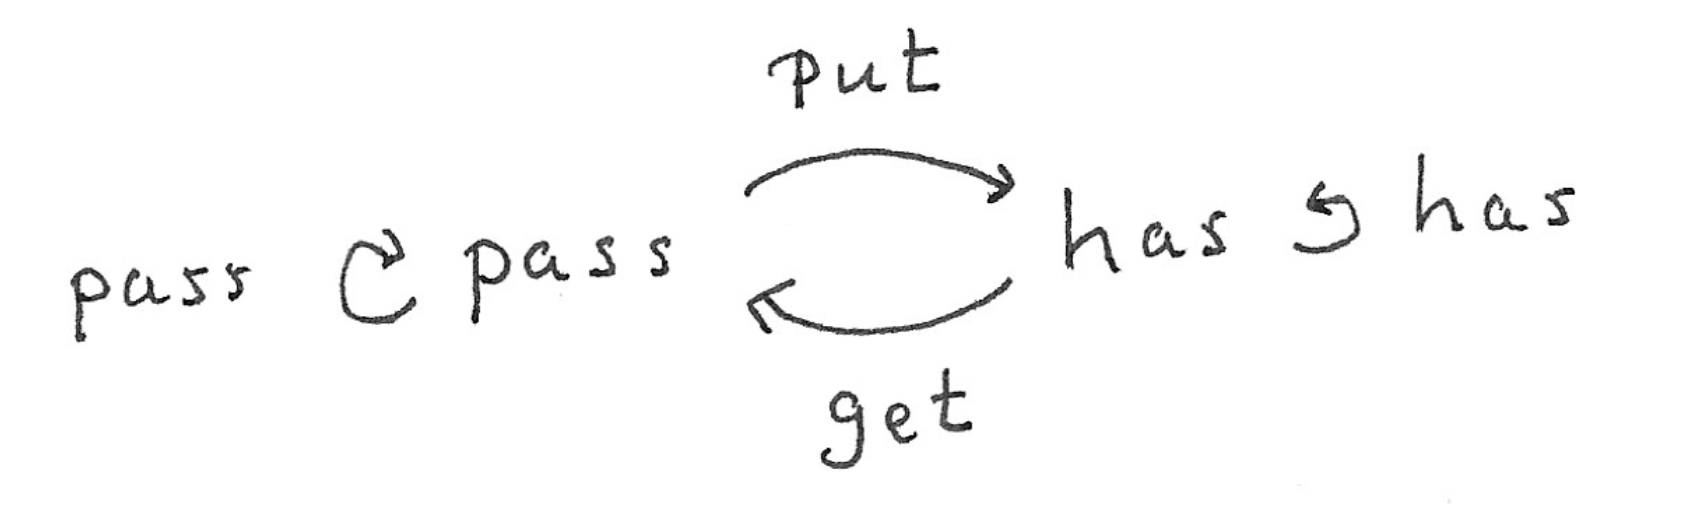
\includegraphics[width=0.55\textwidth]{has.png}
\caption{{\it The spaces {\bf pass} and {\bf has} are isomorphic via $X\leftrightarrow (:X)$.  A similar isomorphism exists for each atom type.  This shows that the space of all pure data 
is isomorphic to a subspace of itself for each atom type.}}
\end{figure}

The space pass is the ``garden'' where we will search for the simplest, most ``organic'' spaces.  
The fact that the ``organic natural numbers'' are the only algebraic homomorphisms of pass makes them particularly interesting, and the first candidates to investigate.

\section{Organic Numbers}

      As we have seen, the natural numbers organically as sequences of identical atoms, so we might think of (:) (:) (:) or (a a a) as ``3'', depending on a conventional choice.  
Thus, to study natural numbers, we want to find a space $N$ where the data of the space contains one sequence for each natural number.  There are many 
spaces which do this, for example,  
\begin{itemize}
\item [1)] The space (atoms) contains all sequences of (:) atoms, (), (:), (:) (:),$\dots$. 
\item [2)] The space (ap const a) contains (), a, a\ a, a\ a\ a,\dots. 
\item [3)] The space (is a), also containing (), a, a\ a, a\ a\ a,\dots.
\end{itemize}
Choices 1) and 2) are compatible in the preorder sense, however 3) is not compatible with the others and, for instance, has a different kernel.  
The main point, however, is that 1) 2) and 3) are isomorphic and they therefore have the same semiring structure.  To be definite, let $N$ be the space (is $a$).  
     
     The first thing to notice about $N$ is that it's main structure is natural number addition, since ($N$:$X$\ $Y$) is the natural number sum of ($N$:$X$) and ($N$:$Y$).  
Since homomorphisms are distributive, a homomorphism $f$ of $N$ is defined by $f:a$, and, thus, $f$ is multiplication by some natural number, 
for instance, (ap const $a$\ $a$\ $a$) is multiplication by $3$.  Since homomorphisms are distributive morphisms, they automatically distributes over addition in $N$.  
Since the group of units is just the identity 1, all of the homomorphisms are central.  
     
    Subspaces of $N$ are indicated by subspace morphisms.  As always, the subspace $1$ is the whole of $N$ and the subspace $0$ consists of just the neutral data of $N$, which, 
since in is distributive is the empty sequence.  The following are easily verified to be classes subspace morphisms as well.  
\begin{itemize} 
\item [1.] {\bf Saturation subspaces} An morphism which computes, for example, min($n$,2) such as (min a a), is a subspace containing the three data \{(), a, a a\}. 
\item [2.] {\bf Modular arithmetic subspaces} An morphism which removes three (a) atoms while possible, such as (while rem $a$ $a$ $a$) is a subspace which computes the sum of it's inputs modulo 3.  Note 
that (while rem a a a) contains the same data as (min a a), but they have a completely different algebraic structure.  
\end{itemize}
These two unsurprising subspaces have a slightly more surprising generalization.  For $p,q\ge 1$, let rem($p$,$q$) be the morphism defined by 
\begin{equation}
{\rm while}\ n\ge p,q: {\rm remove\ p\ from\ n}
\end{equation}
The rem(p,q) are also subspaces and modular sum and saturation cases since rem($p$,$p$) is $n\mapsto n$ mod $p$ and rem($1$,$q$) is $n\mapsto$ min($n$,$q-1$).   General arguments $p,q\ge 1$.  The rem subspaces are closed under composition via 
\begin{equation}
{\rm rem}(p,q)\cdot {\rm rem}(p',q') = {\rm rem}({\rm LCM}(p,p'),{\rm max}(q,q'))
\end{equation}
where {\it LCM} is the least common multiple.  This makes the rem a closed commutative semilattice of subspaces of N.  
This completes the subspace analysis of N since we can show that every subspace of N is either the whole of N, a constant, or is rem(p,q) for some $p,q\ge1$. 

\begin{proof}
Let $f:{\mathbf N}\rightarrow{\mathbf N}$ where $f(x+y)=f(f(x)+y)=f(x+f(y))$ for all $x,y\in\mathbf N$...
\end{proof}

At this point, it is quite possible to consider pairs of natural numbers representing, say, the pair (3,2) as (n a a a : a a) or (n: (:a a a) (:a a)).  Rather than doing this, however, we 
first want to investigate the most organic generalizations of (is a), for instance, (is a b), which we refer to as N$_2$.  
As with the case of N, let's consider subspaces of N$_2$.  

\begin{itemize}
\item{The subspaces 1 and 0 give the whole of N$_2$ and just the empty sequence as subspaces, respectively.  
Projections N$_2$$\cdot$(is a)$\cdot$N$_2$ and N$_2$$\cdot$(is b)$\cdot$N$_2$ produce two N-isomorphic subspaces.}
\item{Lexical sorting of N$_2$ sequences is a non-distributive subspace of N$_2$.  Call this endomorphism N$_2$.lex, the data of N$_2$.lex 
can be written $a^m b^n$ for $m,n\ge 0$.  As in the previous case, a homomorphism M of N$_2$.lex is defined by  
\begin{itemize}
\item [] $M: a\mapsto a^{m_{11}} b^{m_{21}}$, and 
\item [] $M: b\mapsto a^{m_{12}} b^{m_{22}}$ 
\end{itemize}
for some choice of 
$
\left (
\begin{array}{cc} 
m_{11} & m_{21} \\ m_{12} & m_{22}  
\end{array}
\right ) 
$
so the action of M is matrix multiplication.  Thus, the data of N$_2$.lex are pairs of natural numbers the 
homomorphisms are ${\rm Mat}_{2\times2}(\mathbf N)$.  The automorphisms of N$_2$.lex are 
$
\left (
\begin{array}{cc} 
1 & 0 \\ 0 & 1 
\end{array}
\right ) 
$
and 
$
\left (
\begin{array}{cc} 
0 & 1 \\ 1 & 0 
\end{array}
\right ) 
$
and the central products are the matrices 
$
\left (
\begin{array}{cc} 
m & n \\ n & m 
\end{array}
\right ) 
$
for $m,n\in\mathbf N$.


}
\item{Reducing data in N$_2$ by removing (a b) and (b a) subsequences defines another subspace (N$_2$.reduce) consisting of 
sequences containing only a's or only b's but not both.  It is easy to see that data in N$_2$.reduce can be identified with 
ring of integers $\mathbf Z$.  The action of the subspace itself does integer addition.  
The two automorphisms of N$_2$.reduce are the identity and the endomorphism which 
swaps $a\leftrightarrow b$.  A homomorphism $f$ is determined by $f:a$, since $f:b$ is determined by commuting with swap. 
Thus, the central homomorphisms of N$_2$.reduce are exactly integer multiplication, distributing over addition since homomorphisms are 
distributive.  

} 
\end{itemize}

FIX ME.... For instance in (is a b c d), one can reduce to a subspace by (a b)=(b a)=(c d)=(d c)=1, this reduction commutes with a lexical sort 
and so the two can be composed to create $\mathbf Z\times\mathbf Z$ with homomorphisms ${\rm Mat}_{2\times2}(\mathbf N)$. 

\subsection{Number Sequences}

      Given the space $N$ from the previous section, let $\mathbb{N}$ be 
\begin{equation}
{{\rm ap}\ ({\rm put\ {\rm n}})\cdot N \cdot ({\rm get\ {\rm n}})}
\end{equation}
where `n' is some chosen atom.  Since $({\rm put\ n})\cdot N \cdot ({\rm get\ n})$ is idempotent, ${\mathbb N}$ is a distributive space containing 
sequences of $n$-atoms containing $N$-data, such as 
\begin{equation} 
{\rm T = (n:a\ a\ a)\ (n:)\ (n:a\ a)\ (n:a)\ (n:)}
\end{equation} 

Unlike the case of N, the action of ${\mathbb N}$ is merely to concatenate sequences.  It's easy, however, to identify 
natural number sum again as one of several subspaces 
\begin{itemize}
\item sum:T = (n:a a a a a a)
\item sort:T = (n:) (n:) (n:a) (n:a a) (n:a a a)
\item min:T = (n:)
\item max:T = (n:a a a)
\item first:T = (n:a a a)
\end{itemize} 
All but the last are algebraic subspaces and, predictably, have established names.  
Some morphisms of ${\mathbb N}$ can be ``inherited'' from $f\in$N.  Define inner:F to be 
\begin{equation}
{\mathbb N}\cdot({\rm put\ n})\cdot {\rm F}\cdot({\rm get\ n})\cdot{\mathbb N}
\end{equation}
so that (inner:F):X means letting F act on the concatenated N-contents of $X$, returning the result in a single n-atom.  The sum morphism 
above, for instance, is equal to inner:N.  The construction of Equation 7 works for any space, and so we can define a ``functor'' {\it Seq} to be 
\begin{equation}
({\rm put}\ {\rm A})\cdot {\rm B} \cdot ({\rm get}\ {\rm A})
\end{equation}
Then {$\mathbb N$} is equal to (Seq n:N) and given any atom s and any space S, (Seq s:S) is the space of S-values stored in s-atoms.  
Similarly, if we define {\it inner} to be  
\begin{equation}
{\mathbb N}\cdot\{({\rm put\ n})\cdot{\rm B}\cdot({\rm get\ n})\}\cdot{\mathbb N}
\end{equation}
then inner:F is the inner version of F$\in$S.  Other general constructions of this type are possible.  For example, let {\it series} be 
\begin{equation}
{\mathbb N}\cdot\{{\rm B\ (A:B)}\}\cdot{\mathbb N} 
\end{equation}
and, thus (series:F) applies F to data appending the result.  For example, the morphism series$\cdot$(inner:back a a)
generates the Fibbonacci sequence (n:a) (n:a) (n:a a) (n:a a a)$\dots$.

\begin{figure}[h]
\centering
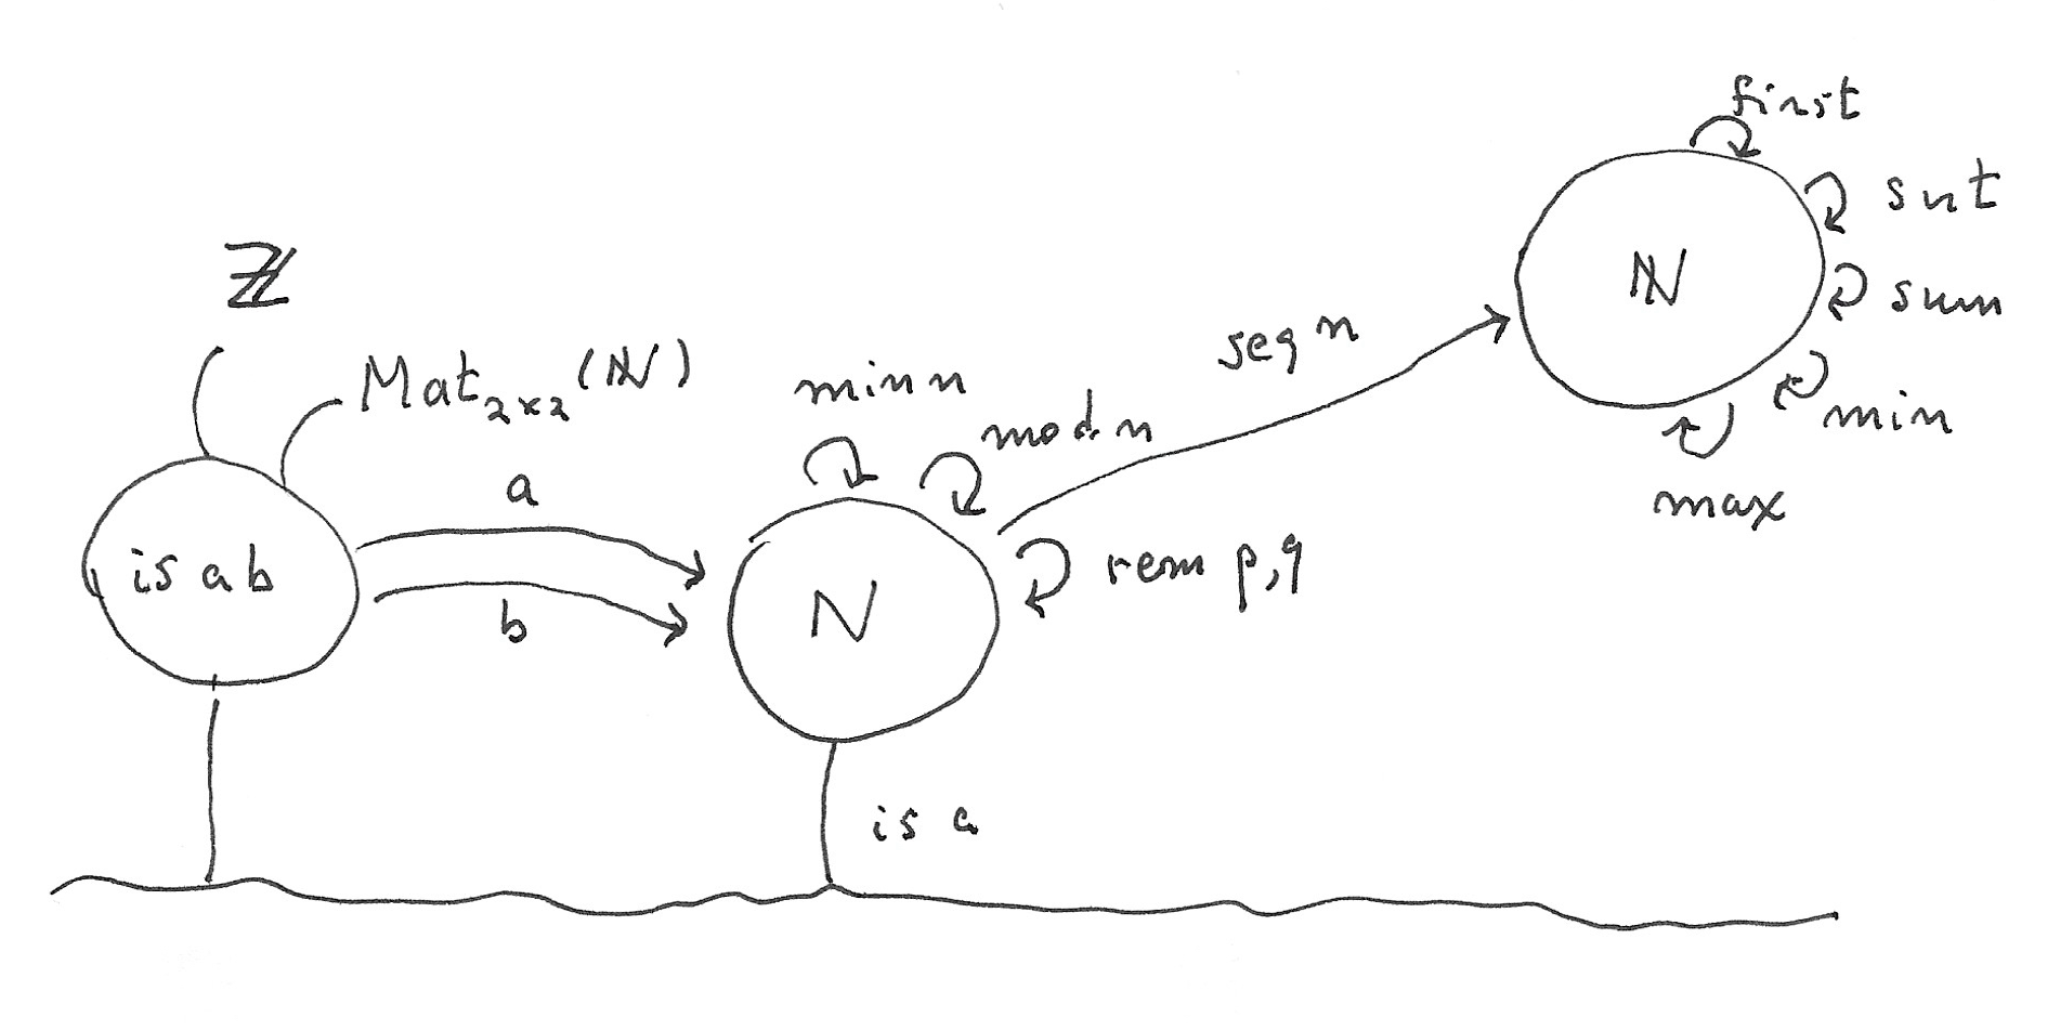
\includegraphics[width=0.7\textwidth]{organics.png}
\caption{{\it Organic numbers.}}
\end{figure}

Exploring further in this vein is certainly possible.  It's worth keeping in mind that if spaces commute, their commutator is a new space.  

COMPLEX NUMBERS? QUATERNIONS?  ANY MORE SURPRISES? SEQUENCES, real numbers, calculus, etc... 

This pretty clearly can be done.  The main question is does this reveal insights or new structures?  

A very natural question, for instance, is what mathematical structures can be represented as subspaces of (is a b c$\dots$)?  

\section{Boolean} 

      The space `bool' is algebraic and neutral, but not distributive.  Since bool contains two data:  () for {\it true} and (:) for {\it false},   
 bool has only four morphisms:  the identity ID=bool, two constants: TRUE=\{\} and FALSE=\{(:)\}, and one involution 
 NOT=bool$\cdot$not$\cdot$bool.  The morphism semiring is explicit in Table X, where it's useful to note that $\oplus$ is commutative since {\bf bool} is 
 algebraic, and $f\oplus f=f$ for $f\in${\bf bool}.  

\begin{table}
\begin{tabular}{| l | l | l | l | l |  }
$f\cdot g$ & ID & TRUE & FALSE & NOT  \\
\hline
ID &  ID & TRUE & FALSE &  NOT \\
TRUE & TRUE & TRUE  & TRUE & TRUE \\
FALSE & FALSE  & FALSE & FALSE & FALSE   \\
NOT & NOT & FALSE & TRUE & ID \\
\hline
\end{tabular}
\begin{tabular}{| l | l | l | l | l |  }
$f\oplus g$ & ID & TRUE & FALSE & NOT  \\
\hline
ID &  ID & ID & FALSE & FALSE \\
TRUE & - & TRUE  & FALSE & NOT \\
FALSE & -  & - & FALSE & FALSE   \\
NOT & - & - & - & NOT \\
\hline
\end{tabular}
\caption{{\it Product and sum of the four morphisms ID, TRUE, FALSE, NOT of the space bool}.  Note that ID is the unit of multiplication and TRUE is the 
unit of addition, and we have $f\oplus g=g\oplus f$, since bool is algebraic, and $f\oplus f=f$.}
\end{table}

The subspaces of bool are ID, TRUE and FALSE, so bool has only trivial subspaces.  The morphisms ID and TRUE are neutral, ID is the only positive 
morphism and all morphisms are algebraic since bool itself is algebraic.  The group of units is ID and NOT, and ID is the only central morphism. 

\subsection{Boolean Sequences}

As in the case of N, we can let $\mathbb L$=(Seq b:bool), be the distributive space of bool-valued data stored in b-atoms, so a typical data in $\mathbb L$ is 
\begin{equation}
{\rm (b:)\ (b:)\ (b:(:))\ (b:)\ (b:(:))\ (b:(:))}
\end{equation}
Let's agree to write such sequences replacing (b:) with T, (b:(:)) with F and the empty sequence with 0, so that the above is written TTFTFF.   
Let's also consider the shortest subspaces of $\mathbb L$ first.  The space morphism {\bf first}$\in\mathbb L$ are the sequences of length at most 1.  
Let's call this space ${\mathbb L}_1$ and, similarly, let ${\mathbb L}_2$ be (first 2)$\in\mathbb L$.  
Thus, ${\mathbb L}_1$ contains data \{0,T,F\} and ${\mathbb L}_2$ contains data \{0,T,F,TT,TF,FT,FF\}. 
For ${\mathbb L}_1$, we can specify a morphism $f\in {\mathbb L}_1$ by listing the values of $f$ on 0,T,F in standard order, so, for example, `0TF` denotes the identity morphism. 
Since ${\mathbb L}_1$ has 27 morphisms, we can be completely explicit about this space.  Table X shows the semiring of morphisms and Figure Y shows special 
properties.  Even with relatively small space like ${\mathbb L}_1$, all the classes of morphisms appear in a nontrivial way.

\begin{figure}[h]
\centering
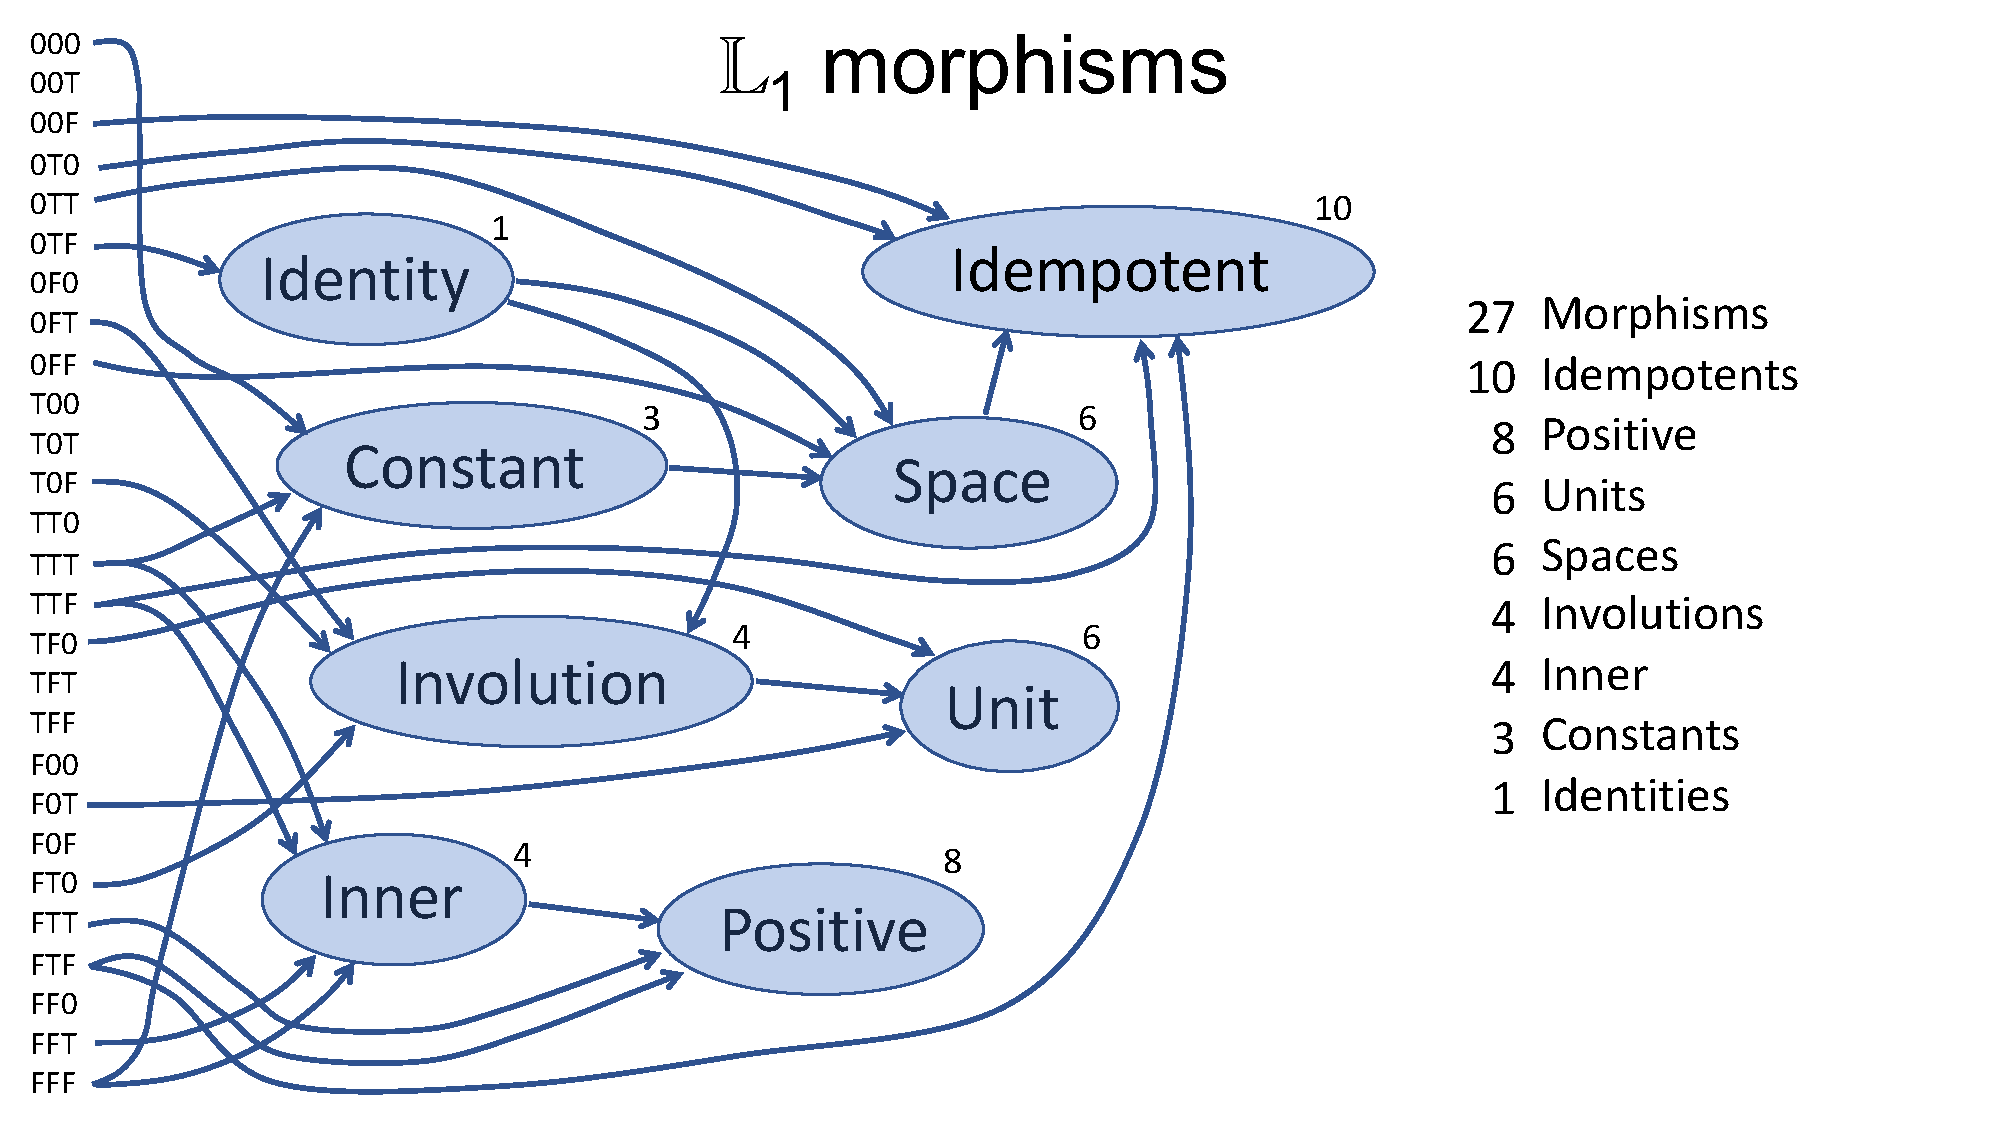
\includegraphics[width=0.8\textwidth]{L1.pdf}
\caption{{\it Morphisms of ${\mathbb L}_1$.}}
\end{figure}

    Moving to ${\mathbb L}_2$, there are already $7^7=823,543$ morphisms; far too many to be as explicit as in the case of ${\mathbb L}_1$.  One simple attempt is to examine just the inner morphisms, since there are only eight of these consisting of 
 the morphisms ${\mathbb L}_2\cdot ({\rm put}\ b)\cdot {\rm F} \cdot ({\rm get}\ b) \cdot {\mathbb L}_2$
for some data F.  These eight depend only on the total number of (:) values in the b-atoms of input, and each morphism returns exactly one b-atom.  
The inner morphisms of ${\mathbb L}_2$ are all algebraic homomorphisms, so we may expect them to be
mathematically interesting.   

\begin{table}
\caption{The eight inner morphisms of ${\mathbb L}_2$ slightly generalize the eight standard symmetric binary boolean operators.}
\centering 
\begin{tabular}{r c c c c c c c r r l}
\hline\hline
$e_i \in {\mathbb L}_2$ & 0 & T & F & TT & TF & FT & FF & standard & generalized & description \\ [0.5ex] 
\hline
$e_1$  & T & T & T & T & T & T & T & TRUE & {\bf always} & always true \\
$e_2$  & T & T & T & T & T & T & F & OR & {\bf any} & any are true \\
$e_3$  & T & T & F & T & F & F & T & XNOR & {\bf even} & even (:)s \\
$e_4$ & T & T & F & T & F & F & F & AND & {\bf all} & all are true \\
$e_5$ & F & F & T & F & T & T & T & NAND & {\bf notall} & not all are true \\
$e_6$ & F & F & T & F & T & T & F & XOR & {\bf odd} & odd (:)s \\
$e_7$ & F & F & F & F & F & F & T & NOR & {\bf none} & none are true  \\
$e_8$ & F & F & F & F & F & F & F & FALSE & {\bf never} & never true \\
\hline
Number of (:)   & 0 & 0 & 1 & 0 & 1 & 1 & 2 &  \\ 
\hline
\end{tabular}
\label{table:L2}
\end{table} 

Table Y shows the eight morphisms and their values on \{0,T,F,TT,TF,FT,FF\}.  Looking at the values for the last four entries \{TT,TF,FT,FF\} 
we recognize that these are slight generalizations of the eight standard symmetric binary boolean operators.  The values of the eight morphisms 
on \{0,T,F\} suggests that the standard binary operator names (`OR' as opposed to `any') are not particularly illuminating in this larger context.  

\section{Summary, Outlook, Rewrite Framework} 


\begin{figure}[h]
\centering
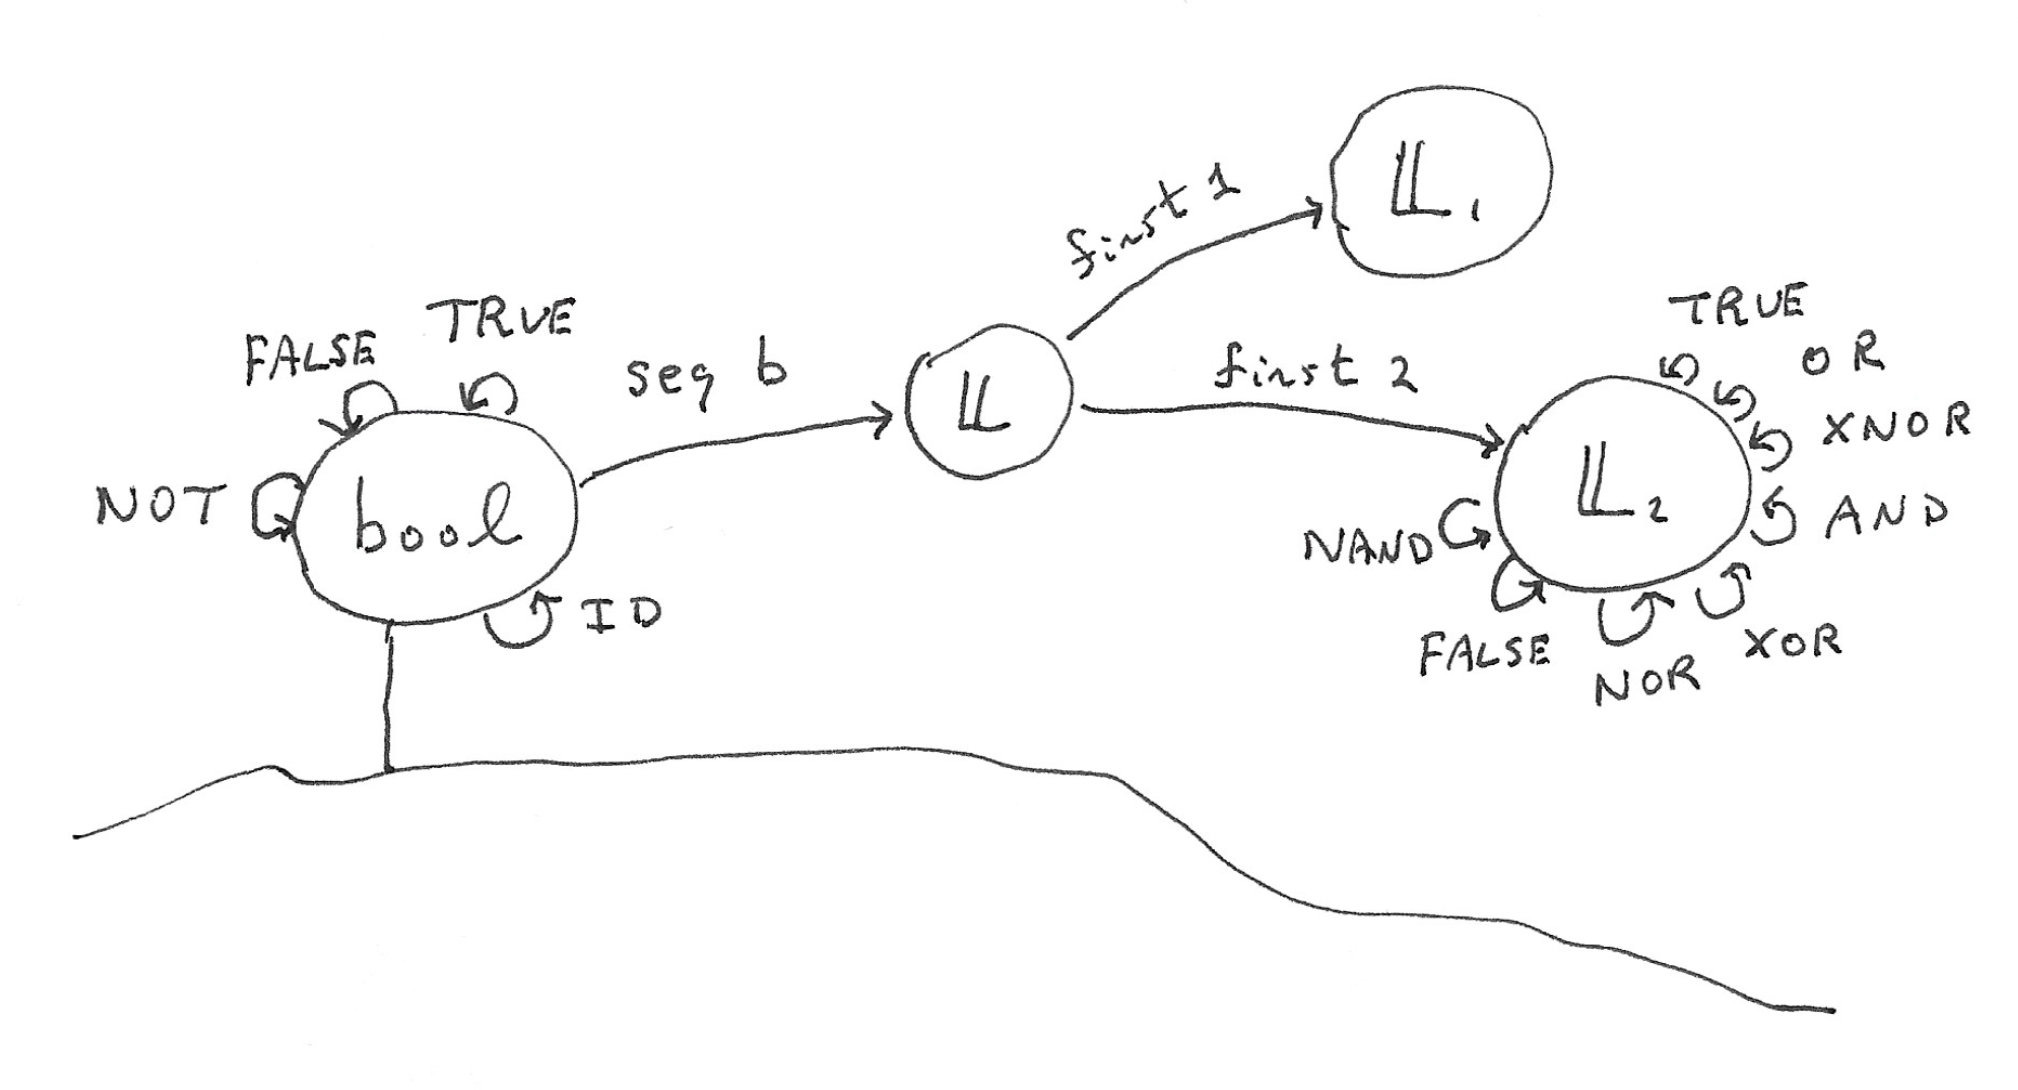
\includegraphics[width=0.8\textwidth]{bool.png}
\caption{{\it A summary of the boolean spaces discussed in the text.  {\bf bool} is the most organic - the space of two boolean values () for true and (:) for false.  The space $\mathbb L$ is sequences of such values with subspaces of at most one (${\mathbb L}_1$) and at most two (${\mathbb L}_2$) values.}}
\end{figure}


\section{Glossary}

\begin{enumerate}
\item {Basics
\begin{enumerate}
\item{$\delta_{\rm const}$ : (const A : B) $\mapsto$ A)}
\item{$\delta_{\rm put}$ : (put A : B) $\mapsto$ (A:B)}
\item{$\delta_{\rm get}$ : (get : (:B)) $\mapsto$ B....FIXME}
\item{$\delta_{\rm atoms}$ : (atoms : b B) $\mapsto$ (:)\ (atoms : B)}
\item{$\delta_{\rm bin}$ : (bin A:B) $\mapsto$ (bin A:B), atom}
\end{enumerate}
}
\item {Control
\begin{enumerate}
\item{$\delta_{\rm if}$: (if ():B) $\mapsto$ B }
\item{$\delta_{\rm if}$: (if a A:B) $\mapsto$ () }
\item{$\delta_{\rm while}$: (while A:B) $\mapsto$ B if (A:B)=B }
\item{$\delta_{\rm while}$: (while A:B) $\mapsto$ (while A: A : B) }
\end{enumerate}
}
\item{Sequence 
\begin{enumerate}
\item{$\delta_{\rm first}$ : (first : b B) $\mapsto$ b}
\item{$\delta_{\rm first}$ : (first : ()) $\mapsto$ ()} 
\end{enumerate} 
}
\end{enumerate}

%%%%%%%%%%%%%%%%%%%%%%%%%%%%%%%%%%%%%%%%%%%%%%%%%%%%%%%%%%%%%%%%%%%%%%%%
%%% 
\begin{thebibliography}{10}
\bibitem{PDF} {\it Pure Data Foundation of Mathematics and Computing}, Saul Youssef, 2023.
\bibitem{Berry} Nicholas Griffin (2003-06-23). {\it The Cambridge Companion to Bertrand Russell}. Cambridge University Press. p. 63. ISBN 978-0-521-63634-6.
\bibitem{Mazur} Barry Mazur, {\it When is one thing equal to some other thing?}, Harvard University, 2007,  {\rm https://people.math.harvard.edu/}$\sim${\rm mazur/preprints/when\_is\_one.pdf}. 
\end{thebibliography}
%%%%%%%%%%%%%%%%%%%%%%%%%%%%%%%%%%%%%%%%%%%%%%%%%%%%%%%%%%%%%%%%%%%%%%%%
\end{document}
